%%%Módulo 3:
%% Carga vertical y horizontal genérica de un cohete (ejemplo White 3.12, página 158, pero en vez de tiro vertical, tiro oblicuo) (C)
\item Considere un cohete con propulsión a chorro en vuelo con una inclinación $\theta$
como se muestra en la figura \ref{fig:cohete}. Utilizando balances integrales
de momento lineal, calcule la fuerza resultante sobre el cohete (considerando
también la gravedad y el efecto del chorro propulsor). Liste todas las hipótesis
utilizadas y exprese la solución en términos generales, es decir, en forma
de ecuaciones:
\begin{equation*}
F_x = F_x(\theta, \dot{m}, \vec{V}_{c}, \vec{V}_{e}, \rho)
\qquad \qquad
F_y = F_y(\theta, \dot{m}, \vec{V}_{c}, \vec{V}_{e}, \rho, \vec{g})
\end{equation*}
\\
Extienda la formulación anterior para el caso en que haya viento. Integrando la expresión que obtuvo para la fuerza, dé una expresión genérica del alcance del cohete si este parte con una inclinación $\theta_0$, con una masa de combustible $m_0$, suponiendo un flujo másico constante $\dot{m} = m_0/t_{vuelo}$.
\begin{figure}[h!!!!]
  \centering
  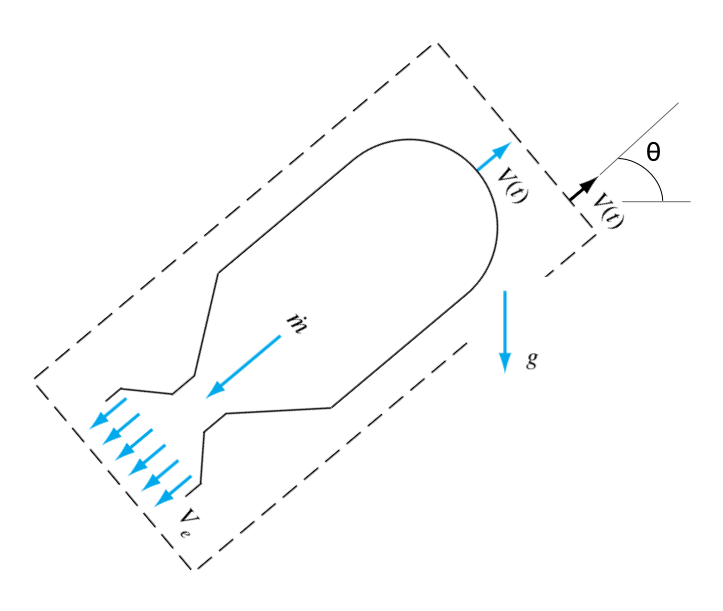
\includegraphics[width=0.5\textwidth]{rocket.png}
  \caption{Cohete en vuelo a velocidad $V(t)$ con inclinación $\theta$}
  \label{fig:cohete}
\end{figure}
